\documentclass[10pt]{article}         %% What type of document you're writing.

%%%%% Preamble

%% Packages to use

\usepackage{amsmath,amsfonts,amssymb}   %% AMS mathematics macros
\usepackage{graphicx}
\usepackage{lmodern}  % for bold teletype font
\usepackage{amsmath}  % for \hookrightarrow
\usepackage{xcolor}   % for \textcolor
\usepackage{listings}
\lstset{
  basicstyle=\ttfamily,
  columns=fullflexible,
  frame=single,
  breaklines=true,
  postbreak=\mbox{\textcolor{red}{$\hookrightarrow$}\space},
}

%% Title Information.

\title{HomeWork 03}
\author{Deep Dand}
%% \date{2 July 2004}           %% By default, LaTeX uses the current date

%%%%% The Document

\begin{document}

\maketitle

\begin{abstract}
Pocket algorithm, Linear Regression(applied as classification method) on Blob dataset
\end{abstract}

\section{Problem}
\subsection{a}
This is the output with PLA $$w=0$$
Code Begins
\lstinputlisting{blob_pocket_pla_w_0.py}
Code ends
\\Output\\
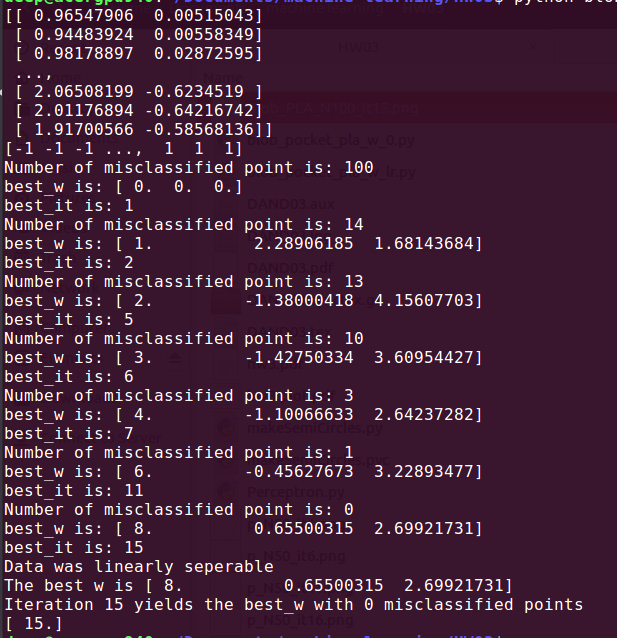
\includegraphics[scale=0.45]{Blob_PLA1}
\\The plot looks like, 
\\
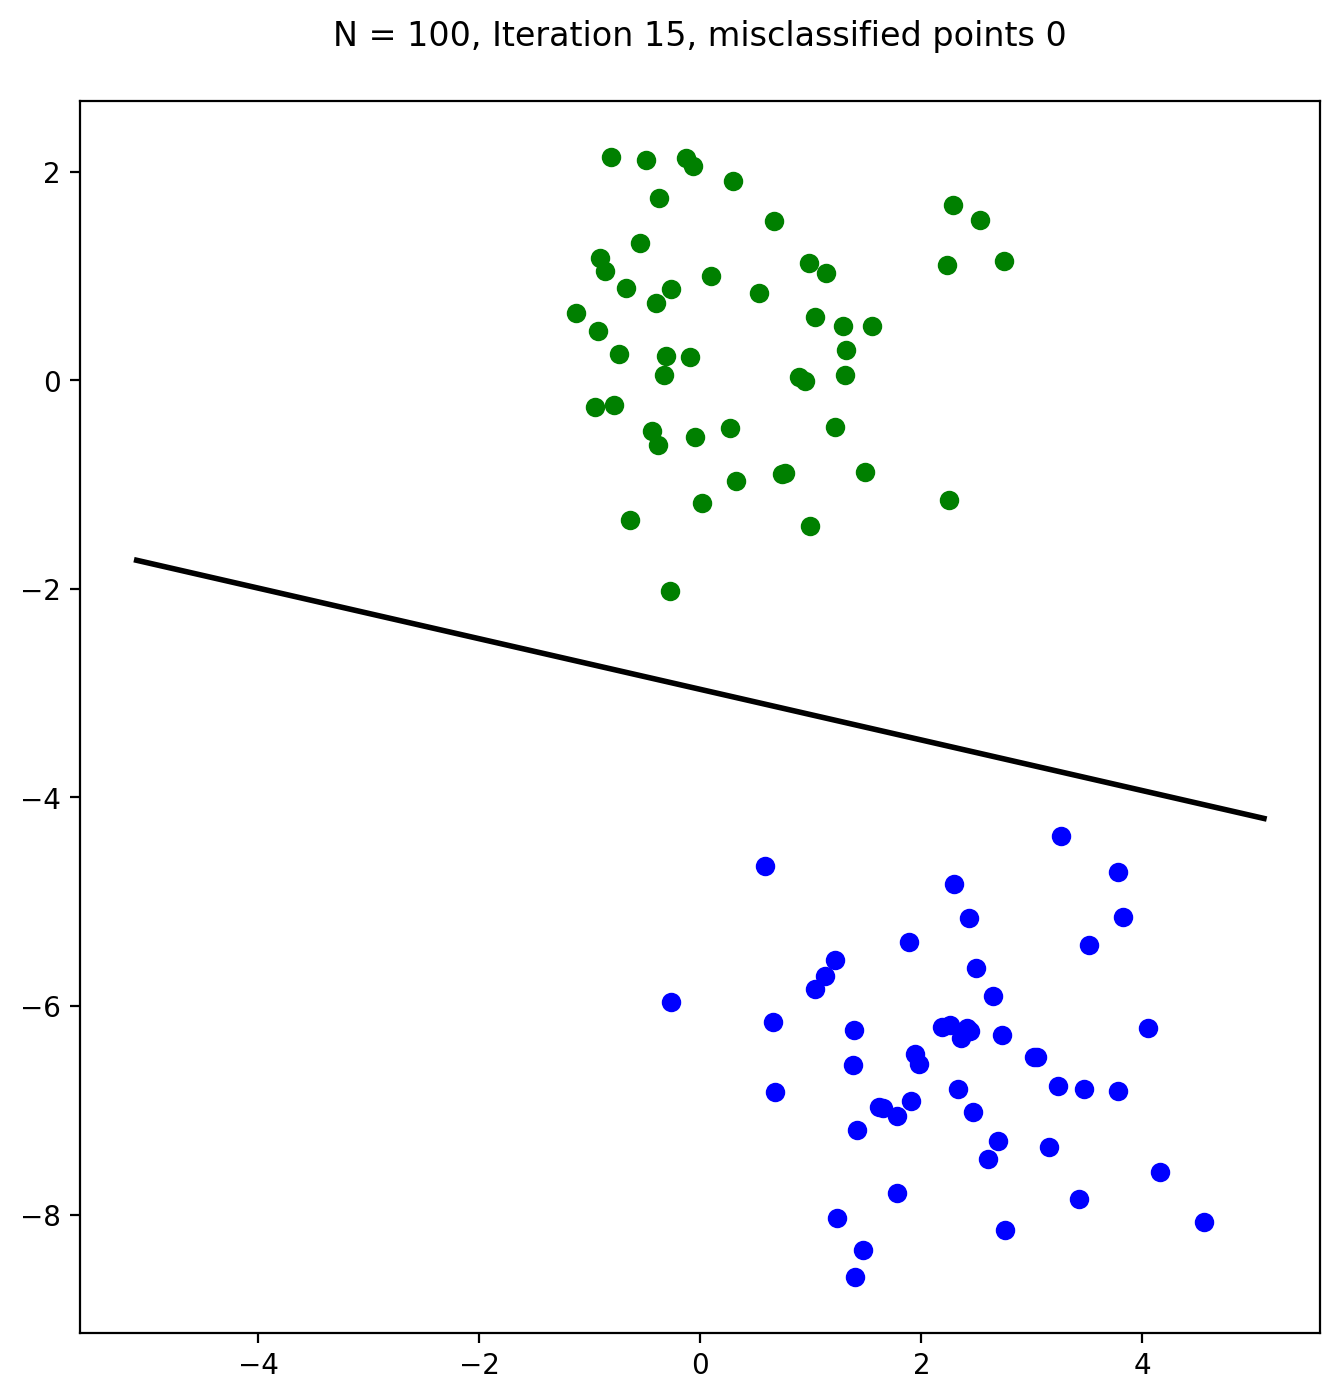
\includegraphics[scale=0.45]{Blob_PLA_N100_it15}
\\The pocket algorithm takes 15 iterations for the execution time and finds the best classification. The best weight is $$w = [8,  0.655, 2.6699]$$ and the best result came at iteration 15.
\subsection{b}
The output of Linear regression weights-
Code Begins
\lstinputlisting{blob_pocket_pla_w_0.py}
Code ends. 
\\Output\\
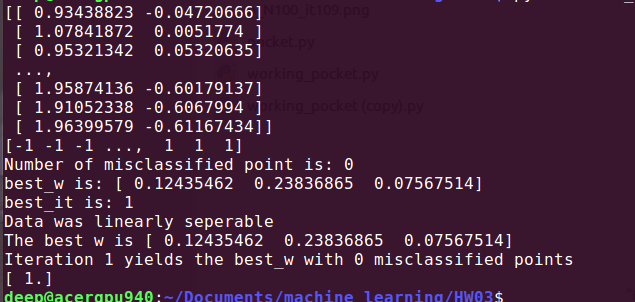
\includegraphics[scale=0.45]{Blob_LR1}
\\The plot looks like, 
\\
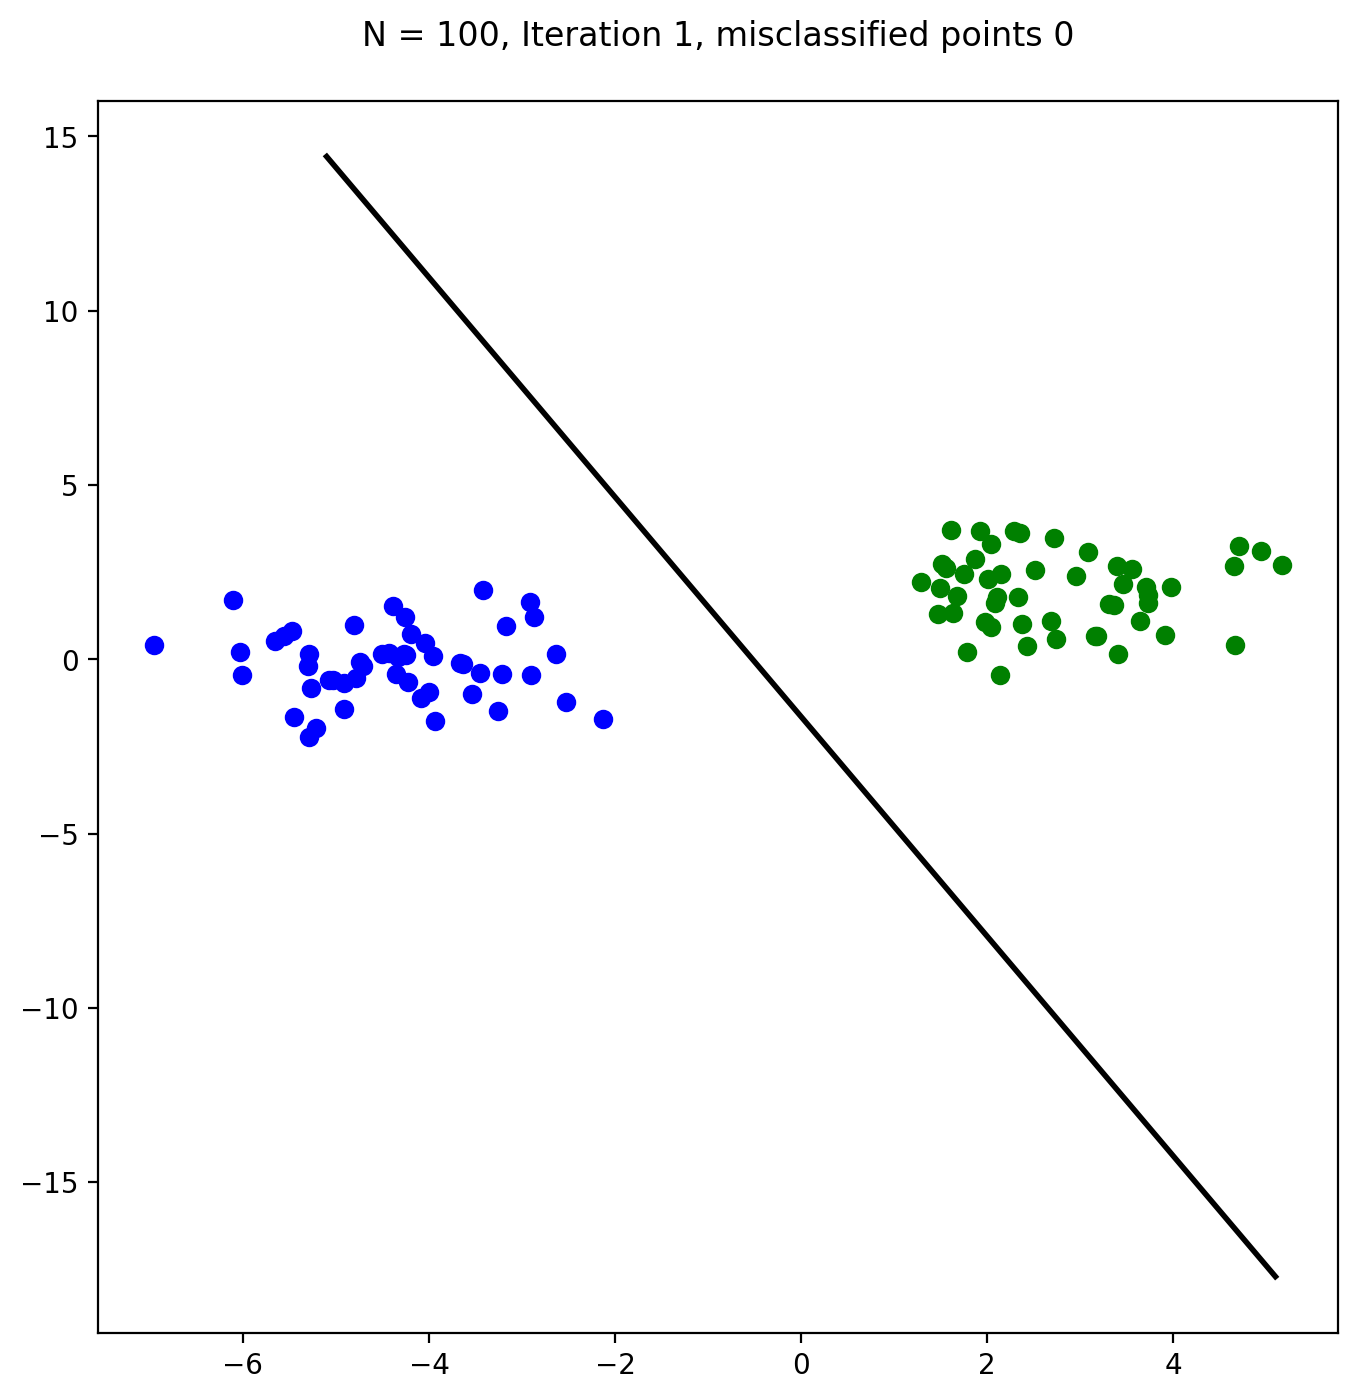
\includegraphics[scale=0.45]{Blob_LR_N100_it1}
\\The linear regression takes only 1 iterations for the execution time and finds the best classification. The best weight is $$w = [0.1243,  0.2383, 0.0757]$$ and the best result came at iteration 1.

\section{summary of experiments}
From the experiments that we have performed in this document, linear regression weights are a good way to initialize the weights for pocket algorithm/PLA. The Linear regressions itself aren't the best at giving goof accuracy but if the weights from LR is given as initial weight to Pocket Algorithm, the results can be much faster to converge since initializing the results to some potential value helps Pocket to identify the closest possible results in less number of iterations.

\end{document}

